\documentclass{report}

\usepackage{graphicx}
\usepackage{hyperref}

\title{G9 Impulse-NG}
\author{Se-Joon Chung \and Wenxun Huang \and Chun Yang \and TA: Zuofu Cheng}
\date{Fall 2010 \\ \hfill \\ ECE 395: Advanced Digital Projects Lab \\ University of Illinois at Urbana-Champaign}

\renewcommand\thesection{\arabic{section}}
\renewcommand\thesubsection{\arabic{section}.\arabic{subsection}}

\begin{document}
\maketitle
\newpage

\section*{Abstract}
\addcontentsline{toc}{subsection}{Abstract}
Project G9 Impulse-NG is a derivation from the G9 Impulse: Video Game 
System project by Zuofu Cheng, James Cavanaugh, Eric Sands, Sean Bires, 
and Chris Schmich during the Fall 2005 and Spring 2006 semesters. As 
the original gaming system was a project from almost 5 years ago, this 
project's aim was to import the whole system to more modern hardware 
platform and extend its capabilities. The Altera DE2 was chosen as the
target platform due to ECE students' relative familiarity with said
platform. Due to obstacles encountered and time constraints, a complete
port of the system remains unfinished. The G9 Impulse-NG currently
only supports drawing a single frame with alpha blending for drawing
sprites.

\tableofcontents
\newpage

\section{Project Description and Overview}
\subsection{G9 Impulse (The Original System)}
The original G9 Impulse was an 8-bit, 2D gaming system. It can use an NES 
controller or custom arcade controls as input and outputs to a CRT
monitor at a 320x240 resolution using interlacing 
mode. It has 2-bit DAC for each of the red, blue, green colors, 
allowing a total of 64 colors. Audio is provided through an MP3 player 
via standard 3.5mm audio jack. For further details, please take a look 
at the original G9 Impulse report at 
\url{https://courses.engr.illinois.edu/ece395/projects/spring2006/project9\_final\_paper.doc}.

\subsection{G9 Impulse-NG}
The G9 Impulse-NG is still an 8-bit, 2D gaming system, but with extended 
hardware capabilities. It uses the Altera DE2 FPGA board which supports 
10-bit DAC video out for each of the red, blue, green colors as opposed 
to the 2-bit DAC on the original system. Also, it is designed to output 
to an LCD monitor without interlacing at a 640x480 resolution. Currently, it does 
not support audio.

\subsection{Tools Used}
The primary tool used in this project was the Quartus II 9.1/10.0 which 
can be downloaded from the Altera website. It was used to compile the VHDL 
code and to program the Altera DE2 board. Also, the MegaWizard Plug-In 
Manager and NIOS II SOPC Builder under the tools tab in Quartus II were 
used to generate some of the required entities. ModelSim-Altera 6.5b 
Starter Edition, which can also be downloaded on the Altera website, was 
used to simulate the entities and aid in debugging.

In terms of hardware, the project utilized the Altera DE2 Development 
and Education Board for the GPU and the PIC18F4620 as the CPU.

\subsection{Description of GPU Components}
Most of the work was done on the Altera DE2 FPGA board which is the 
graphics processing unit of the game system. The following are the 
components inside the GPU chip on the Altera DE2 board.

\subsubsection{GPU Chip (gpuchip.vhd)}
The gpuchip is the top level entity inside the Altera DE2 board. It 
takes instructions through the pin\_port\_addr and pin\_port\_in ports
as inputs from an external PIC18F4620 microprocessor (CPU) and marshals
the information to be used as operands for the blitter. When the blitter
operation is done, the gpuchip signals back to the PIC that the
operation has been completed.

To use the gpuchip, appropriate registers must be loaded with all the information 
required by the blitter to begin its operations. As the data port is only 8-bits wide,
the information is passed from the PIC to the gpuchip in multiple cycles. One should
load pin\_port\_addr with the address of the register and the 
pin\_port\_in with the data, then raise the pin\_load to signal the
gpuchip to update the register. Table~\ref{tab:gpu_instructions}
 shows the list of addresses and corresponding registers.

\begin{table}[htb!]
    \begin{center}
        \begin{tabular}{ | c | c | }
            \hline
            Address & Register \\
            \hline
            0000-0010 & Source Address MSB-LSB \\
            \hline
            0011-0101 & Target Address MSB-LSB \\
            \hline
            0110 & Source Lines \\
            \hline
            0111 & Line Width in pixels/2 \\
            \hline
            1000 & Alpha Op Register \\
            \hline
            1001 & Double Buffer Enable \\
            \hline
            1010 & Front Buffer Register \\
            \hline
        \end{tabular}
    \end{center}
    \caption{GPU Instruction Set (from G9 Impulse Final Documentation)}
    \label{tab:gpu_instructions}
\end{table}

Figure~\ref{fig:gpu_state_diagram} shows the internal state machine of 
gpuchip. During the INIT state, the blitter is reset for its first time 
use. In the LOAD state, the registers are loaded when the pin\_load is 
high. Then it continues onto the DRAW state when pin\_start is asserted 
high. In the DRAW state, the gpuchip instructs the blitter to begin its 
drawing operations. When the blitter raises the blit\_done signal, the 
gpuchip moves onto the REST state where it resets the blitter once more 
for next usage and signals the PIC that it is ready to accept the next 
command.

\begin{figure}[htb!]
    \begin{center}
        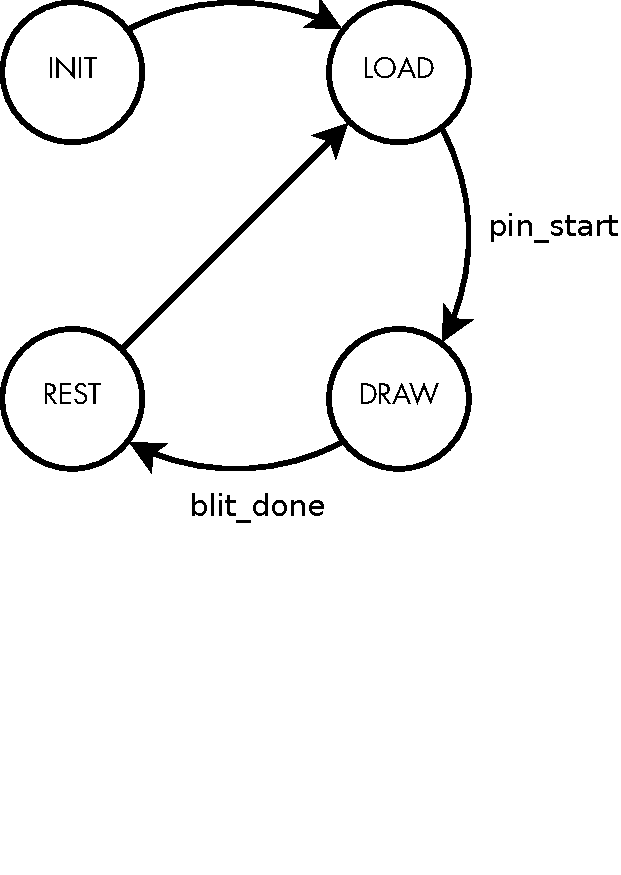
\includegraphics[width=2in,trim=0 2.3in 0 0,clip=true]{gpu_state}
    \end{center}
    \caption{GPU State Diagram}
    \label{fig:gpu_state_diagram}
\end{figure}

Figure~\ref{fig:block_diagram} shows the overall connections inside the gpuchip.
 However, due to connection problems in the hardware wiring 
from the DE2 board to external devices, the current system does not 
utilize the connections between the PIC18F4620 microprocessor. In
particular, we believe 40-pin connector cable connecting the DE2 board
and the breadboard where the PIC resides does not form a stable
connection. Also, there is crosstalk among the wires of the cable.

\begin{figure}
    \begin{center}
        \vspace{-0.875in}
        
\includegraphics[width=4.5in]{gpu-inside}
    \end{center}
    \caption{Block diagram of G9 Impulse-NG}
    \label{fig:block_diagram}
\end{figure}


\subsubsection{Blitter}
The blitter facilitates transferring large amounts of data in memory,
from the sprite sheet to the framebuffer. Operands for the blitter are
provided by registered inputs from the GPU, which ultimately originate
from the PIC. The blitter uses the operands and reads the appropriate
bytes from the sprite sheet and blits them onto the framebuffer. The
blitter supports alpha blending which enables it to have transparent pixels 
in a square sprite region.

The operands required to operate the blitter are given in
table~\ref{tab:blitter_operands}.

\begin{table}[htb!]
    \begin{center}
        \begin{tabular}{ | c | l | }
            \hline
            Operand & Description \\
            \hline
            Source Address & Address in sprite sheet to blit from \\
            \hline
            Target Address & Address in framebuffer to blit to \\
            \hline
            Source Lines & Number of rows to blit \\
            \hline
            Line Width in pixels/2 & Width of each row (divided by two
            because each \\
            & word in the SDRAM stores data for two pixels) \\
            \hline
            Alpha Op & Whether or not to enable alpha blending \\
            \hline
            Front Buffer & Specifies which framebuffer to draw to \\
            \hline
        \end{tabular}
    \end{center}
    \caption{Blitter Operands}
    \label{tab:blitter_operands}
\end{table}

The architecture of the G9 Impulse-NG was redesigned and resembles the
original G9 Impulse blitter only in function and I/O. Originally, the
sprite sheet and framebuffer both existed in the SDRAM. However, due to
complications in reading and writing to the SDRAM without a
dualport module for the Altera SDRAM controller, the SRAM was used to hold the
 framebuffer. Using the SRAM also has the advantage of
simplicity and speed, as writes to the SRAM can be completed within one
clock cycle. As the SRAM must also be used by the view entity to calculate
the appropriate colors to output to the VGA device, so access to the
SRAM must be arbitrated. To make sure there are no conflicts in using
the SRAM, the view entity sends a sram\_waitrequest to block writes while
the screen is being drawn. Particularly, since the VGA is only drawing the
framebuffer to the upper left quadrant of the screen, the blitter is
allowed to write when the VGA is drawing the bottom half of the screen.
Figure~\ref{fig:blitter_waitrequest} shows when the blitter is allowed
to write to SRAM.

\begin{figure}[htb!]
    \begin{center}
        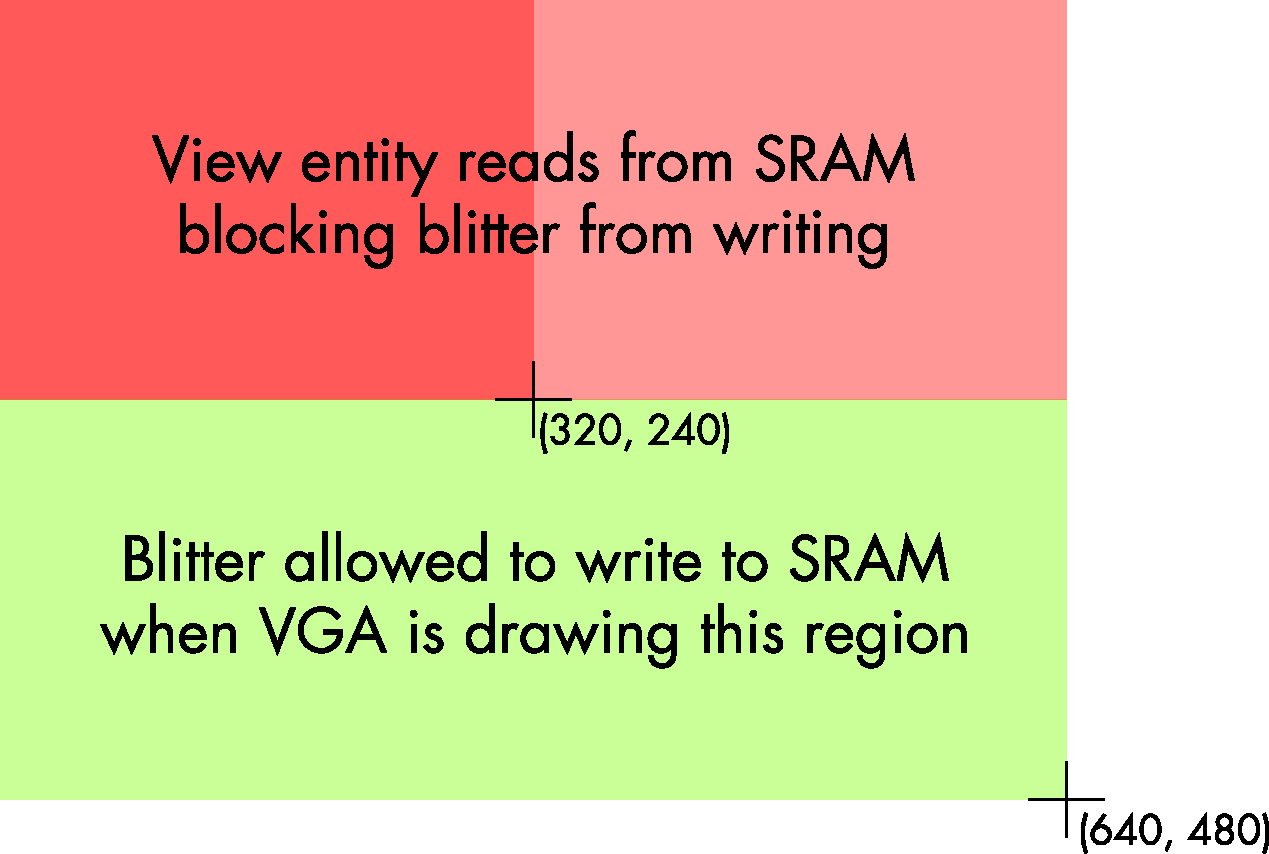
\includegraphics[width=4.5in]{blitter_waitrequest}
    \end{center}
    \caption{How SRAM access from blitter and view is divided}
    \label{fig:blitter_waitrequest}
\end{figure}

The blitter is comprised of two processes and a queue. One of the
processes reads sprites from the sprite sheet and puts the data into the
queue. The other process reads from the queue and writes the data into
the framebuffer when the blitter is given permission to do so. A diagram
of the interaction is given in figure~\ref{fig:blitter_process}.

\begin{figure}[htb!]
    \begin{center}
        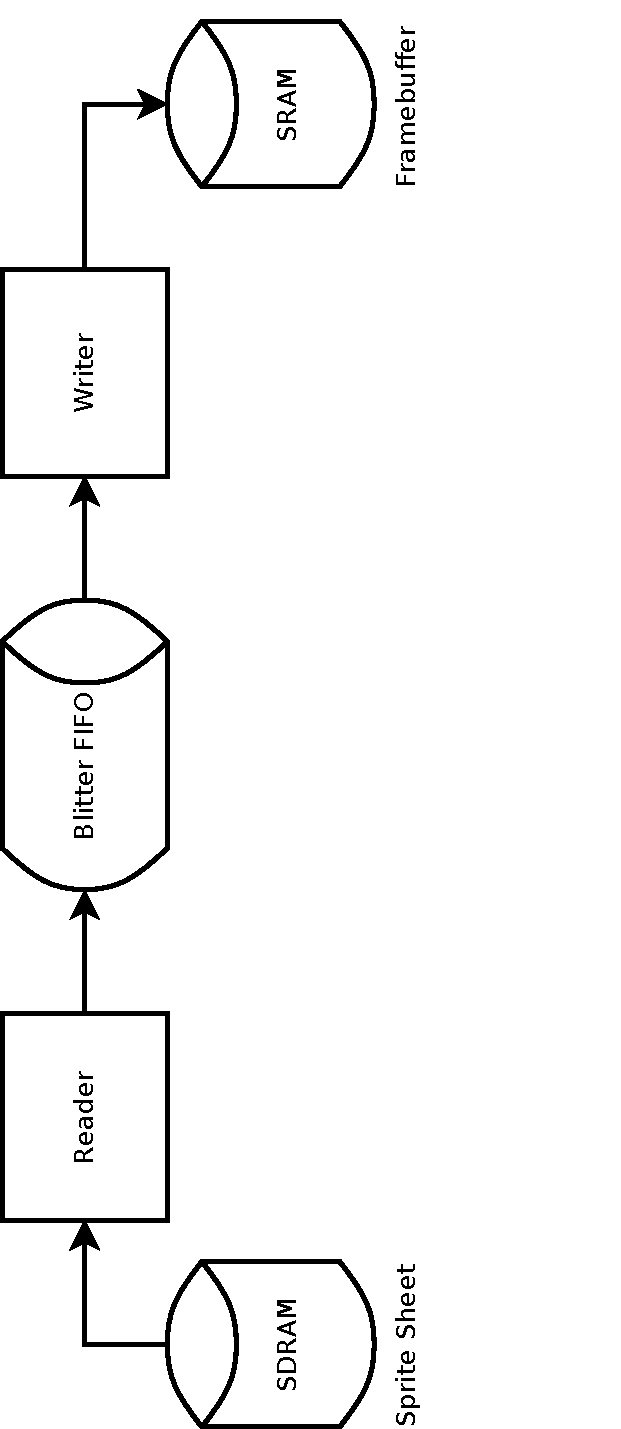
\includegraphics[angle=270,width=4.5in,trim=0 0 1in 0,clip=true]{blitter_process}
    \end{center}
    \caption{Diagram of how the blitter works}
    \label{fig:blitter_process}
\end{figure}

This design was chosen to take advantage of being able to
read from the sprite sheet and write to the framebuffer simultaneously.
In the original G9 Impulse, this was not possible because both
operations would involve accessing the SDRAM, but since the G9
Impulse-NG uses the SRAM for the framebuffer, using this architecture
results in a slight speed increase because reads and writes can occur
simultaneously.

Since reads from the SDRAM are pipelined, data is available several
cycles after a read is issued. Using the queue allows the blitter to
catch all the data read from the SDRAM independent of whether the writer
is able to write the data immediately. When the VGA is drawing the
screen, the writer will be blocked from accessing the framebuffer. With the
queue in place, though, the reader will still be able to read from the
sprite sheet until the queue is full.

Again, because of pipelining, data may arrive even after read is
deasserted. Thus, the queue must always have enough room to accept the
data. Therefore, an `almost full' signal determines whether or not reads
are allowed.

State diagrams for the blitter is given in
figure~\ref{fig:blitter_state}.

\begin{figure}[htb!]
    \begin{center}
        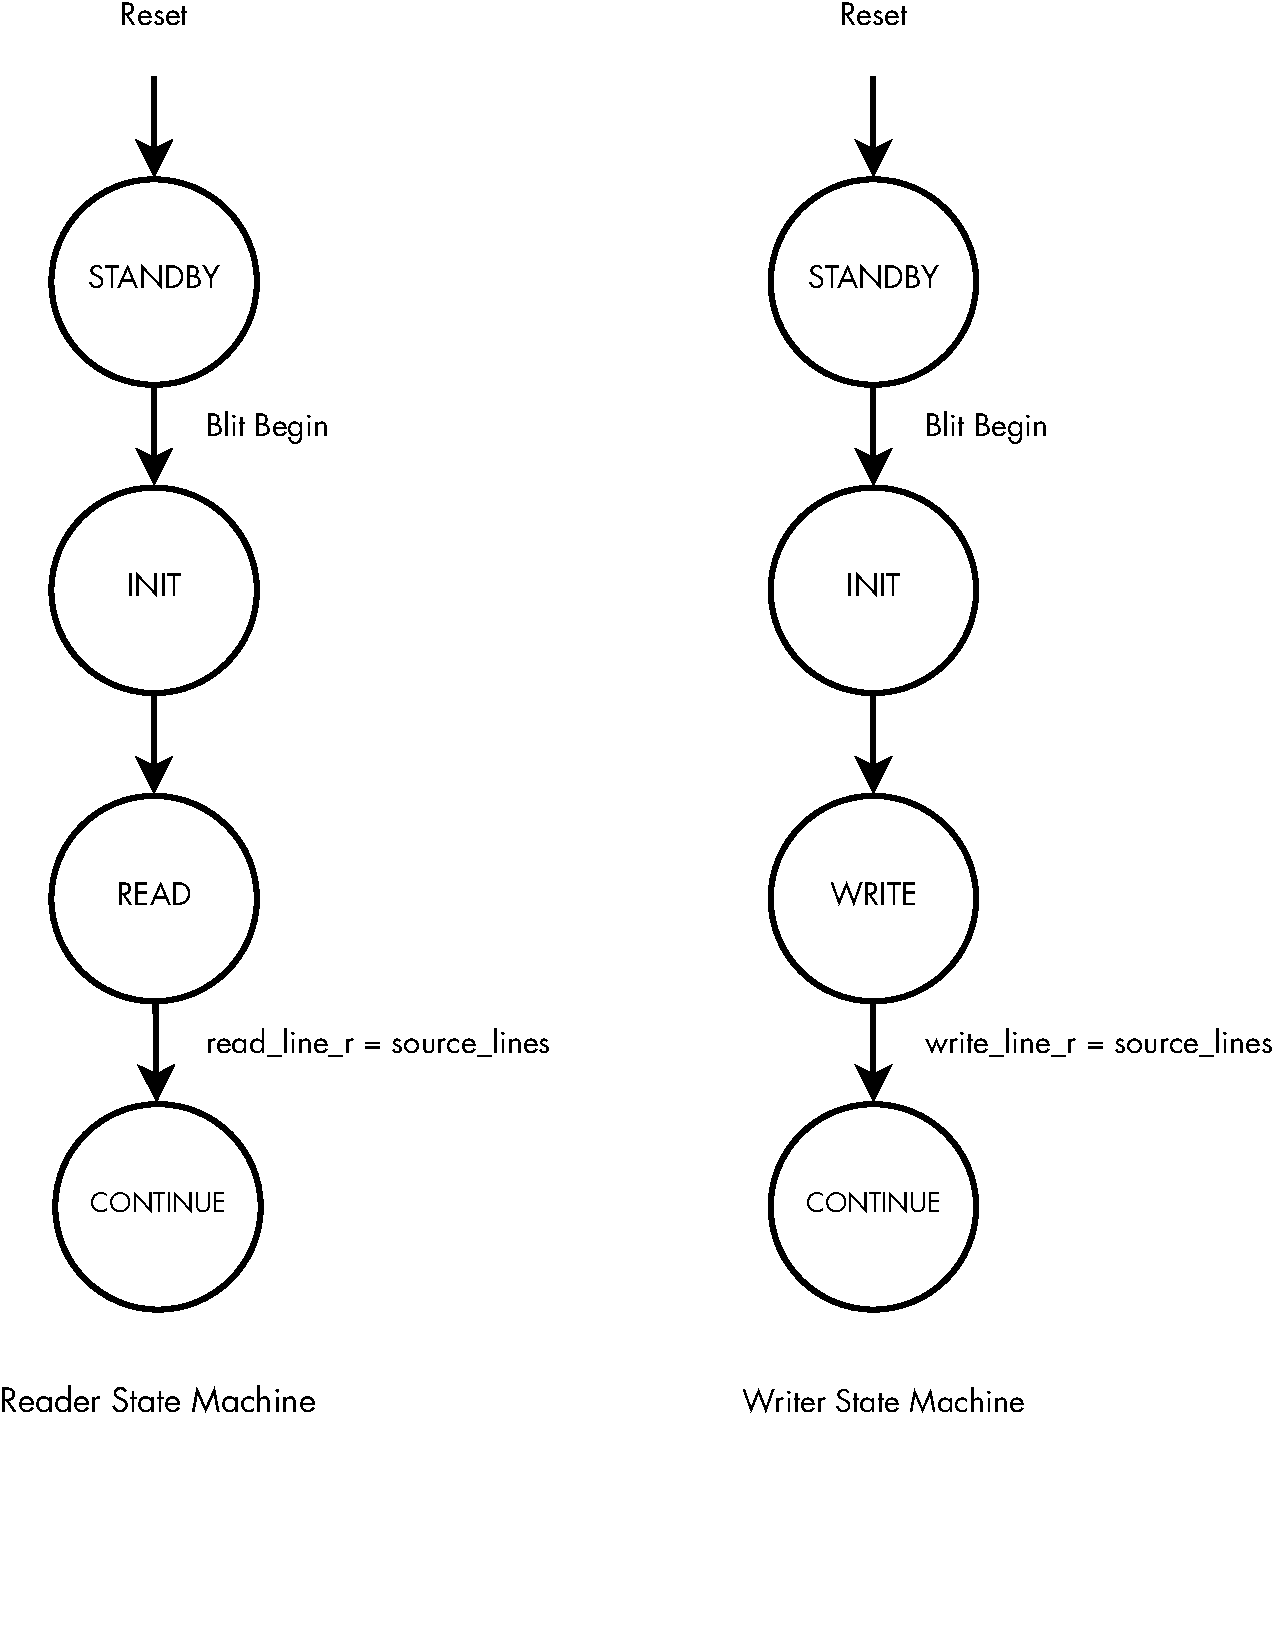
\includegraphics[width=4.5in,trim=0 1.5in 0 0,clip=true]{blitter_state}
    \end{center}
    \caption{Blitter state diagrams}
    \label{fig:blitter_state}
\end{figure}

The two processes behave almost identically except for the direction of data
flow and the conditions which allow the process to operate. When in the
STANDBY state, the two processes wait for the blit\_begin signal to
begin processing. Upon receiving the signal, various registers are
loaded/reset with information about the source address, target address,
current row being read/written, and current position being read/written
in the current row. During the READ and WRITE states, the two processes
respectively read from the sprite sheet and write to the framebuffer.
Reads occur when the queue is not full and the SDRAM waitrequest is not
asserted. Writes occur when the queue is not empty and the SRAM
waitrequest is not asserted. Both processes finish when the number of
lines read/written is equal to the number of source lines.

Due to two pixels being stored in each sprite sheet address, the
original G9 Impulse implemented alpha blending by reading both from the
framebuffer and from the sprite sheet and blitting one or both pixels
based on the color and the value of the alpha op operand. The Xilinx
SDRAM controller used by the G9 Impulse did not support writing and
reading to only one byte of the two byte memory location. The SRAM used by the G9
Impulse-NG however does support a byte enable signal. Thus, the G9
Impulse-NG blitter is able to perform alpha blending without reading
back from the framebuffer. The result of this is that when blitting large
sprites with alpha blending on, the new blitter will be faster because
there will be less memory accesses.

When finished blitting, the blitter asserts the blit\_done signal. To
blit another sprite, the blitter must be reset. The logic inside the
GPU chip takes care of handling the blit\_done signal and resetting the
blitter between operations.

\subsubsection{Blitter FIFO (blitter\_fifo.vhd)}
The blitter fifo entity is a 512-byte, First-In First-Out buffer created 
by the Altera MegaWizard tool. It is implemented on the M4K memory block 
on the FPGA board. The buffer keeps track of current level of usage. 
Using this information, it signals the blitter when it is allowed to read and
write.

\subsubsection{View (view.vhd)}
The view entity handles outputs to the LCD monitor. It generates the 
vertical sync, horizontal sync, and blank signals for the LCD monitor to 
use and the appropriate RGB values that go with the current pixel 
position on the screen. The view entity uses the on-board asynchronous 
SRAM as the framebuffer for fast access and allows the blitter to write to the SRAM 
when the SRAM is not being read. The subcomponents of the view entity 
include the VGA controller (VGA\_controller.vhd) and Color Mapper 
(Color\_Mapper.vhd).

\subsubsection{VGA Controller (VGA\_controller.vhd)}
The vga\_controller entity takes a 50 MHz clock as its input and 
generates a 25 MHz clock which acts as the pixel clock and the 
appropriate horizontal and vertical sync pulses. It also outputs the 
current coordinates on the screen as DrawX and DrawY. The code is 
sourced from Lab 9 of the ECE 385 (Digital Systems Laboratory) course at 
the University of Illinois at Urbana-Champaign.

\subsubsection{Color Mapper (Color\_Mapper.vhd)}
The Color Mapper entity takes the current coordinates on the screen and 
decides which color to draw on the screen. Currently, the G9 Impulse-NG 
outputs at a 640x480 resolution, but it only uses the upper left
quadrant of the screen (320x240) for actually displaying the game,
virtually keeping the same resolution as in the original system. The 
Color Mapper outputs the actual game if the current pixel is in the 
upper left quadrant. Otherwise, it just outputs a blue color.

\subsubsection{Dualport RAM (ram2port.vhd)}
The ram2port entity is a 512-byte, 2-port memory block created by the 
Altera MegaWizard tool. It uses the onchip M4K memory and supports 
simultaneous reads and writes. It is used inside the fifo\_cc entity to 
implement a First-In, First-Out buffer.

\subsubsection{FIFO (fifo\_cc.vhd)}
The fifo\_cc entity is a 512-byte, First-In First-Out buffer that uses 
the ram2port entity as its component. It keeps track of current level of 
usage. Originally, the blitter utilized the blitter FIFO to queue pixel 
data. However, a bug was discovered to be fixed when the fifo\_cc was 
utilized instead. Both FIFOs provide signals to tell the blitter when 
reads and writes are allowed.

\subsubsection{Hex Display Driver (HexDriver.vhd)}
The HexDriver entity takes 4-bit number as its input and outputs a 7-bit 
vector that can drive the onboard 7-segment display. The code was 
sourced from ECE 385 class. This entity is not an integral part of the 
GPU and was used only for debugging purposes.

\subsubsection{Phase-Locked Loop (sdram\_pll.vhd)}
The sdram\_pll is the phase-locked loop entity to ensure proper delay 
between the system clock and the SDRAM clock. The SDRAM clock needs to 
be advanced by 3ns with respect to the system clock for it to function 
properly. The PLL entity was generated by the Altera MegaWizard tool.

\subsubsection{SDRAM Controller (sdram\_0.vhd)}
The sdram\_0 entity is the SDRAM controller generated by the NIOS II 
SOPC Builder in Quartus II. It follows the Avalon Memory-Mapped 
Interfaces specification as outlined in 
\url{http://www.altera.com/literature/manual/mnl\_avalon\_spec.pdf}. Out 
of the 22-bit address it takes as input, it uses bits 21 and 8 for the 
bank address, bits 20 down to 9 as the row address, and bits 7 down to 0 
as the column address. One should note that this format for decoding 
address is different from the one they use in the DE2 Control Panel 
program which can be used to write data into the SDRAM. The DE2 Control 
Panel uses bits 21 down to 20 as the bank address, bits 19 down to 8 as 
the row address, and bits 7 down to 0 as the column address. Please look
at Figure~\ref{fig:sdram_address} for the address decoding format.

\begin{figure}[htb!]
    \begin{center}
        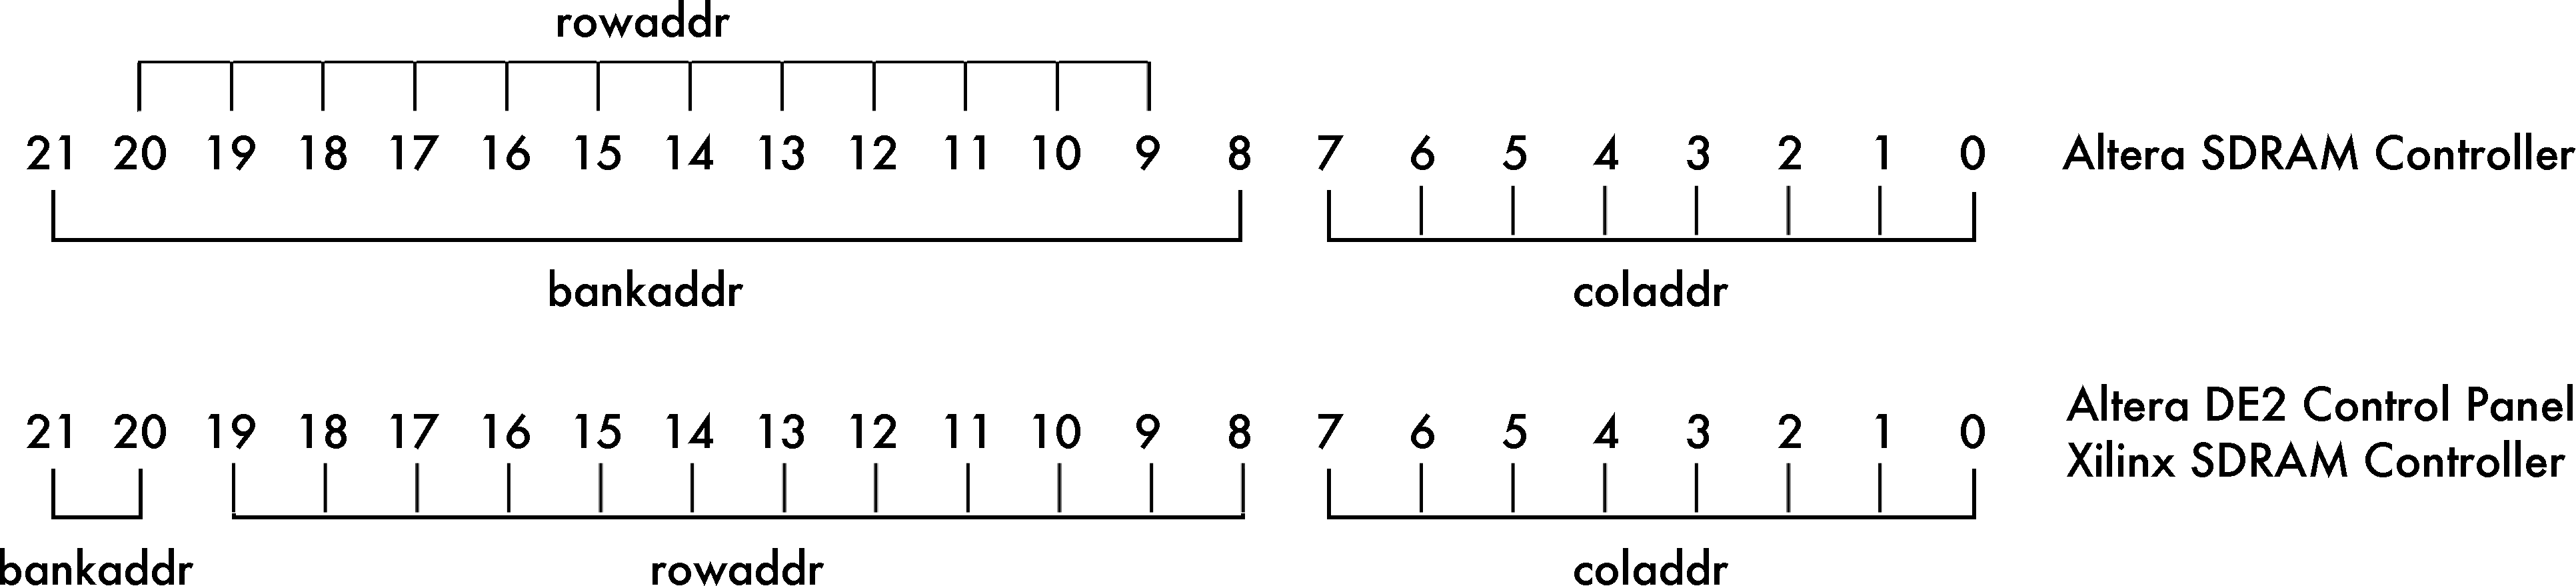
\includegraphics[width=4.5in]{sdram_addresses}
    \end{center}
    \caption{SDRAM Adress Layout}
    \label{fig:sdram_address}
\end{figure}

\subsection{Description of Software Components (Starcell XF-1 Game)}
The original G9 Impulse came with vertical scrolling shooter arcade game 
written for the system titled Starcell XF-1. The game code runs on the 
PIC18F4620 microprocessor which is the main CPU of the system. The game 
code was not actually utilized because of signal crosstalk when wiring 
the DE2 board with the PIC. Particularly, the ribbon cable used to 
connect the 40-pin expansion header on the DE2 board to the protoboard 
which contains the PIC18 and other related components seemed to distort 
and attenuate the signals. However, images from the game was converted 
into a binary file and used extensively in testing functionalities of 
gpuchip.

\newpage
\section{Results}
Most of the time devoted to the project was spent on figuring out how to 
use the SDRAM on the Altera DE2 board. There were no SDRAM controllers 
in VHDL provided by the manufacturer or good documentation on what the 
NIOS II generated SDRAM controller does, so there had been a lot of 
guesswork going into how to use the SDRAM controller. There had also 
been an attempt to use the Xilinx XSB SDRAM controller on the DE2 board, 
but this approach was dropped after realizing that the Altera DE2 board 
does not have hardware support for delay-locked loops. Using ModelSim to 
simulate these controllers aided greatly in having breakthroughs towards 
the end of the semester. After getting the NIOS II controller working, 
it was noticed that the screen was scrambled. The problem was found to 
be the way the address is decoded inside the DE2 Control Panel which is 
used to initialize contents of the SDRAM is different from the way the 
address is decoded inside the SDRAM controller which reads out of the 
memory. After fixing this issue, the vga entity and the blitter was redesigned to 
integrate the corrected usage of the SDRAM controller, but there was not enough time 
left for debugging the glitches in the synchronization between 
components. Also, the PIC18F4620 hardware had to be left out of the 
picture because of bad connection cable. The blitter contains a bug that 
causes the writer to never reach the CONTINUE state, though on screen, 
the blit appears to be completed. We speculate the bug could be caused 
by reading and writing to a nearly empty queue at the same time.  
Perhaps the issue can be fixed by having the blitter writer only operate 
when the queue size is above a minimum threshold. Due to the 
aforementioned problems, the current G9 Impulse-NG hardware can display 
a static frame alpha blended onto the framebuffer.

\section{Future Development}
As it has been discovered how to access the SDRAM and other required 
components inside the gpuchip, if the synchronization issue between 
these components can be resolved, it should be relatively easy to 
display a scrolling background and draw sprites that move around. Audio 
may be added using the onboard support for an audio output. However, it 
has not been tested if the expansion headers can be used to correctly 
receive external inputs into the DE2 board, so there may still be some 
difficulty in interfacing the board with a PIC18. Future developers may
consider using Xilinx FPGAs instead because of the quality of documentation
and resources that Xilinx provides.

\clearpage
\phantomsection
\addcontentsline{toc}{subsection}{Bibliography}
\nocite{website:dualport}
\nocite{website:dualport}
\nocite{website:XSA}
\nocite{website:XSB}
\nocite{website:DE2}
\nocite{website:Avalon}
\nocite{website:PLL}
\nocite{website:G9Impulse}
\nocite{website:Using}

\bibliographystyle{plain}
\bibliography{refs}

\end{document}
